% ============================================================================
\chapter{Inovações}\label{cap:inovacoes}
% ============================================================================

Este capítulo isola as inovações do \vapor{}. Cada uma é apresentada com uma \emph{ficha} que responde às cinco perguntas da \autoref{tab:cinco} --- o quê, para quem, para que, por que, como ---, seguida da evidência que a sustenta e do seu limite. O critério de inclusão é exigente: só entra o que (i) não é prática corrente nos sistemas comparáveis do \autoref{cap:relacionados}, (ii) está implementado e testado no repositório e (iii) tem uma medida que poderia ter falhado.

% ----------------------------------------------------------------------------
\section{Numérica canônica portátil}\label{sec:inov-canonica}

\begin{ficha}{Ficha 1 --- Os mesmos bits em todo substrato}
\textbf{O quê.} Uma semântica de ponto flutuante fixa bit a bit para todos os operadores da álgebra, inclusive divisão e funções transcendentais, realizada igualmente em x86-64 (AVX2, AVX-512), AArch64, RISC-V (VLEN 128 a 512), Vulkan e no oráculo.\\
\textbf{Para quem.} Quem precisa que um resultado numérico seja o mesmo em qualquer máquina: auditoria de modelos de IA, ciência reprodutível, risco financeiro regulado.\\
\textbf{Para que.} Para que ``rodei de novo e deu diferente'' deixe de ser possível e para que a comparação entre máquinas vire um teste de igualdade, não de tolerância.\\
\textbf{Por que.} Porque a irreprodutibilidade vem de escolhas arbitrárias (ordem de redução, FMA, implementação de $\exp$), não de limitações físicas; fixadas as escolhas, a igualdade é de graça.\\
\textbf{Como.} Redução em árvore fixa de 16 acumuladores; multiplicação e soma arredondadas separadamente; divisão corretamente arredondada; transcendentais como microprogramas sobre $+$, $-$, $\times$; paralelismo só entre saídas independentes.
\end{ficha}

A literatura de reprodutibilidade numérica oferece duas respostas: somas reprodutíveis por pré-arredondamento ou acumuladores longos \cite{demmel2015}, que custam um fator constante em cada redução, e modos determinísticos de bibliotecas \cite{pytorchdeterminism}, que garantem igualdade só na mesma máquina e na mesma versão. O \vapor{} toma um terceiro caminho: em vez de tornar a soma insensível à ordem, \emph{fixa a ordem} e tira o paralelismo de outro lugar. Um GEMV tem milhares de linhas independentes; processar $R$ linhas por iteração, cada uma com os seus 16 acumuladores, dá paralelismo de instrução e de \textit{threads} sem tocar em nenhuma soma.

\paragraph{Evidência.} A garantia é testada em todas as formas de paralelismo do sistema (\autoref{tab:invariancias}). Cada linha da tabela é um teste que compara bits, não uma tolerância.

\begin{table}[htbp]
\centering
\caption{Invariâncias testadas bit a bit}\label{tab:invariancias}
\small
\begin{tabularx}{\textwidth}{@{}lX@{}}
\toprule
\textbf{a resposta não depende de} & \textbf{como é testado}\\
\midrule
ISA & AVX2, AVX-512, NEON e RVV (sob QEMU) iguais ao oráculo\\
VLEN do RISC-V & 128, 256 e 512 iguais\\
GPU & Vulkan (lavapipe) igual à CPU no modelo inteiro, com amostragem\\
número de \textit{threads} & 1 = 2 = 3 \textit{threads}\\
lote & tokens de uma sequência iguais sozinha ou num lote contínuo, com qualquer fatiamento do \textit{prefill}\\
lugar do cache & KV paginado igual ao contíguo\\
réplica & qualquer réplica dá a mesma resposta; réplicas entre nós de um \textit{cluster} comparadas bit a bit\\
armazenamento dos pesos & bf16 residente igual a f32 sobre os pesos arredondados\\
especulação & saída da decodificação especulativa (linear e em árvore) igual à do alvo sozinho\\
esparsidade & MoE esparso (e em 4 bits) igual ao denso\\
\bottomrule
\end{tabularx}
\end{table}

\paragraph{Limite.} As transcendentais são iguais em todo lugar mas não corretamente arredondadas (1--2~ulps). A garantia é sobre os substratos medidos; um substrato novo precisa passar pela eclusa (\autoref{sec:inov-eclusas}). O texto normalizado depende da versão do Unicode do OTP, registrada mas não eliminada.

% ----------------------------------------------------------------------------
\section{Desempenho sem reassociar}\label{sec:inov-desempenho}

\begin{ficha}{Ficha 2 --- Velocidade que não troca bits}
\textbf{O quê.} Técnicas de desempenho de fronteira --- MoE esparso, cache latente (MLA), janela deslizante em anel, decodificação especulativa em árvore, paralelismo de tensor, GPU residente --- cada uma reformulada para não mudar um bit.\\
\textbf{Para quem.} Operadores de inferência que hoje escolhem entre velocidade e reprodutibilidade.\\
\textbf{Para que.} Para que otimizar não exija revalidar.\\
\textbf{Por que.} Porque cada uma dessas técnicas é, no fundo, uma escolha de \emph{quais} saídas calcular ou \emph{onde} guardar dados, não de \emph{como} somar.\\
\textbf{Como.} MoE por predicação de linha; paralelismo de tensor por coluna com \textit{all-gather} (nunca por linha com \textit{all-reduce}, que reassociaria); especulação que verifica $k+1$ linhas do alvo num passo; janela como cache circular na tabela de blocos.
\end{ficha}

\paragraph{Evidência.} MoE esparso: 2,6$\times$ no \textit{decode}, bits iguais ao denso. MLA latente: 85$\times$ menos memória de cache. Janela em anel: 7,9$\times$ mais sequências a 32\,k tokens. GPU com sessões residentes: 10--12~ms por token contra 72~ms sem sessão, os bits da CPU. GEMV f32 $2048^2$: 2,24$\times$ com 2 \textit{threads} na mesma máquina de 2 vCPUs, sem mudar um bit.

\paragraph{Limite.} O paralelismo de tensor por linha com \textit{all-reduce}, o mais comum na prática, é recusado; o custo é mais tráfego de rede. O GEMV de 4 bits continua limitado por emissão de instruções.

% ----------------------------------------------------------------------------
\section{Compilar sem confiar no compilador}\label{sec:inov-alocacao}

\begin{ficha}{Ficha 3 --- Alocação sem \textit{spill}, conferida por um verificador provado}
\textbf{O quê.} Um compilador que emite bits de cinco alvos sem assembler, sem C e sem LLVM, em que cada alocação de registradores é aceita só depois de conferida por um verificador provado em Lean e extraído para Elixir.\\
\textbf{Para quem.} Pesquisadores de compiladores verificados; equipes que precisam de uma cadeia de compilação auditável e pequena.\\
\textbf{Para que.} Para que a fase mais propensa a erros sutis (alocação) não precise ser confiada.\\
\textbf{Por que.} Provar uma heurística é caro e frágil; provar o verificador é barato e vale para qualquer heurística.\\
\textbf{Como.} \textit{Linear scan} com blocos alinhados e o fator de grupo $g$ (o LMUL do RVV generalizado a todas as ISAs); sem caminho de \textit{spill} --- falta de registrador muda a forma do código; \code{checkAlloc\_sound} em Lean.
\end{ficha}

O ``sem \textit{spill}'' é uma escolha de primeiros princípios. Um \textit{spill} é uma escrita e uma leitura de memória introduzidas pelo compilador, invisíveis no programa-fonte e difíceis de contar no trabalho certificado. Mudando a forma do código (menos linhas por iteração, grupos menores, fronteiras de região), o compilador mantém o trabalho contado exato e o código sempre dentro dos registradores. A consequência medida está no árbitro: o modelo de três tetos acerta o GEMV de 4 bits porque conta as instruções \emph{como emitidas} (\autoref{sec:arq-arbitro}).

\paragraph{Limite.} O verificador extraído é quadrático; compilar programas grandes desenrolados é lento (cerca de 0,6~s por passo e por ISA no Monte Carlo da rodada 0.13).

% ----------------------------------------------------------------------------
\section{Contenção total do código gerado}\label{sec:inov-contencao}

\begin{ficha}{Ficha 4 --- Nenhum byte emitido executa na máquina virtual}
\textbf{O quê.} Todo código gerado roda em processos do sistema operacional com seccomp, W\^{}X e \textit{watchdog}; funções nativas na VM são proibidas por um teste de auditoria.\\
\textbf{Para quem.} Quem serve modelos ou executa código gerado num serviço de longa duração.\\
\textbf{Para que.} Para que um erro do compilador, do \textit{driver} ou da GPU custe uma requisição, não o serviço.\\
\textbf{Por que.} Porque o compilador não é provado inteiro; a contenção limita o que um erro dele pode fazer.\\
\textbf{Como.} Quadros com comprimento prefixado; tabelas dimensionadas pelo quadro; reinício supervisionado; \textit{failover} que não muda bits.
\end{ficha}

\paragraph{Evidência.} As quatro classes de falha (\code{SIGILL}, \code{SIGSEGV}, \code{SIGALRM}, \code{SIGSYS}) são provocadas nos testes; em todas só o worker morre e a unidade seguinte roda. Um ``interpretador seguro'' em função nativa foi \emph{recusado} no escrutínio da diretriz: compartilharia o espaço de endereçamento da VM.

\paragraph{Limite.} O worker é Linux; um worker para macOS (com \code{MAP\_JIT}, sem seccomp) não foi escrito. Sob \code{qemu-user} o seccomp não está disponível (o isolamento por processo continua).

% ----------------------------------------------------------------------------
\section{Certificados portáteis, co-assináveis e transparentes}\label{sec:inov-certificados}

\begin{ficha}{Ficha 5 --- Um certificado que nós independentes reproduzem byte a byte}
\textbf{O quê.} Um certificado Ed25519 da compilação, sem nenhum dado dependente do \textit{host}, codificado em CBOR determinístico, que vários nós podem refazer e co-assinar, e que pode ser ancorado num log de transparência.\\
\textbf{Para quem.} Cadeias de suprimento de modelos; auditores; reguladores (os dossiês mapeiam cada evidência a dispositivos do AI Act europeu e da ISO/IEC 42001, e dizem onde não há nenhuma).\\
\textbf{Para que.} Para que confiar num binário signifique confiar num quórum, não num fornecedor.\\
\textbf{Por que.} Porque um certificado só tem valor se outro verificador independente consegue reproduzi-lo.\\
\textbf{Como.} Trabalho contado em vez de decisão de despacho; CBOR (RFC 8949 §4.2) em vez de \code{term\_to\_binary}; log Merkle RFC 9162 com \textit{checkpoints} C2SP e testemunhas que recusam retrocesso e bifurcação.
\end{ficha}

\paragraph{Evidência.} Payloads idênticos entre nós; verificação de borda em cerca de 2~ms; num dossiê, nenhuma de 209 alterações de um bit é aceita; o verificador do log roda no próprio navegador.

% ----------------------------------------------------------------------------
\section{Eclusas: admissão por medição}\label{sec:inov-eclusas}

\begin{ficha}{Ficha 6 --- Nada entra sem ser medido na fronteira}
\textbf{O quê.} Três eclusas com a mesma forma: a de \emph{modelos} transforma um \textit{checkpoint} num contrato conferido; a de \emph{substratos} mede um acelerador antes de lhe dar programas; a de \emph{documentos} lê arquivos com a proveniência de cada trecho até a página e o \textit{hash}.\\
\textbf{Para quem.} Quem integra componentes de terceiros --- modelos, aceleradores, documentos.\\
\textbf{Para que.} Para que o núcleo não conheça famílias, fornecedores ou formatos, e para que a recusa venha com o motivo e o reparo.\\
\textbf{Por que.} Porque o custo de integração cresce com o que o núcleo precisa saber; uma eclusa concentra esse conhecimento num lugar só.\\
\textbf{Como.} Contratos (\code{:causal\_lm}, \code{:encoder}, \code{:codec}, \code{:map}); adaptadores por dados (JSON), \textit{blueprint} ou topologia; sondas de resposta conhecida com impressão numérica; leitores próprios de zip, PDF, Office, JPEG, CCITT, JBIG2.
\end{ficha}

\paragraph{Evidência.} Os adaptadores novos são conferidos contra o próprio \code{transformers} --- o que achou um defeito real de \textit{rotary} parcial, admitido e calculado errado em silêncio, num caminho de referência. O decodificador JPEG é igual ao libjpeg bit a bit; CCITT G3/G4, ao libtiff; JBIG2, ao jbig2dec (43 de 43 fluxos).

% ----------------------------------------------------------------------------
\section{Uma busca propõe, um verificador decide --- com controles}\label{sec:inov-proponente}

\begin{ficha}{Ficha 7 --- Toda resposta com o seu juiz, todo juiz com o seu controle}
\textbf{O quê.} Um padrão de arquitetura aplicado a domínios inteiros: o procedimento que produz uma resposta (busca, \textit{solver}, modelo de linguagem, pessoa) é separado do que a confere, e cada verificação é acompanhada de um \emph{controle} --- o valor que uma implementação quebrada produziria --- que mostra que ela poderia ter falhado.\\
\textbf{Para quem.} Quem usa saídas de modelos generativos ou de buscas heurísticas e precisa separar sinal de ruído.\\
\textbf{Para que.} Para que ``a saída parece certa'' seja substituída por ``a saída foi conferida, e a conferência tem poder''.\\
\textbf{Por que.} Porque um verificador sem controle pode estar aceitando tudo; e porque a proposta pode vir de qualquer lugar --- inclusive de um modelo de linguagem --- se o juiz for independente dela.\\
\textbf{Como.} Portões calibrados que \emph{recusam existir} se os controles negativos e positivos se sobrepõem; verificações com valor, controle, limiar e veredito; verificadores pequenos (refutações DRUP, KKT, Kirchhoff, Farkas, motor ingênuo); propostas recebidas pelo MCP.
\end{ficha}

O padrão aparece em três níveis. No \textbf{nível de portão}, um detector de ruído (de texto, imagem ou áudio) é ajustado a controles negativos (ruído, sinal embaralhado, repetição) e positivos (sinal real retido) e se recusa a julgar se a margem entre eles for nula. No \textbf{nível de verificação}, a suíte de qualidade (\code{mix vapor.quality}) tem, em cada linha, um controle; na rodada 0.12 foram 147 verificações, todas aprovadas, e a rodada 0.13 acrescenta 23 (\autoref{cap:avaliacao}). No \textbf{nível de domínio}, cada mesa (lógica, engenharia, ciência, finanças) devolve com a resposta um certificado calculado fora do \textit{solver} --- e aceita a \emph{proposta} de qualquer um, conferindo só ela.

\begin{figure}[htbp]
\centering
\begin{tikzpicture}[node distance=6mm and 9mm, font=\footnotesize]
\node[box] (q) {problema\\(texto)};
\node[box, right=of q, yshift=9mm] (s) {busca / \textit{solver}};
\node[box, right=of q, yshift=-9mm] (m) {pessoa ou modelo\\(MCP)};
\node[box, right=of s, yshift=-9mm] (prop) {proposta +\\certificado};
\node[acc, right=of prop] (v) {verificador\\independente\\(pequeno)};
\node[dark, right=of v] (out) {aceito /\\recusado com motivo};
\node[bad, below=8mm of v] (c) {controle:\\o que um juiz\\quebrado aceitaria};
\draw[arr] (q) -- (s); \draw[arr] (q) -- (m); \draw[arr] (s) -- (prop); \draw[arr] (m) -- (prop);
\draw[carr] (prop) -- (v); \draw[carr] (v) -- (out); \draw[arr, dashed] (c) -- node[lbl, right] {deve ser recusado} (v);
\end{tikzpicture}
\caption{O padrão proponente/verificador com controle. A busca pode ser complexa e não confiável; o verificador é pequeno e independente; o controle mostra que ele tem poder.}
\label{fig:proponente}
\end{figure}

\paragraph{Evidência.} Na lógica, a satisfatibilidade de $S(3) = 13$ é decidida com refutação DRUP e a refutação truncada é rejeitada. Na engenharia, o MEF com elemento QM6 fica a 0,9\% da viga analítica enquanto o Q4 trava a 29\% --- e o certificado de equilíbrio é calculado fora do \textit{solver}. Nas finanças, o juiz ingênuo do livro de ofertas achou um defeito real que o motor de produção e o próprio juiz compartilhavam (\autoref{sec:fin-livro}). A \autoref{fig:logica} mostra a mesa de lógica no console.

\begin{figure}[htbp]
\centering
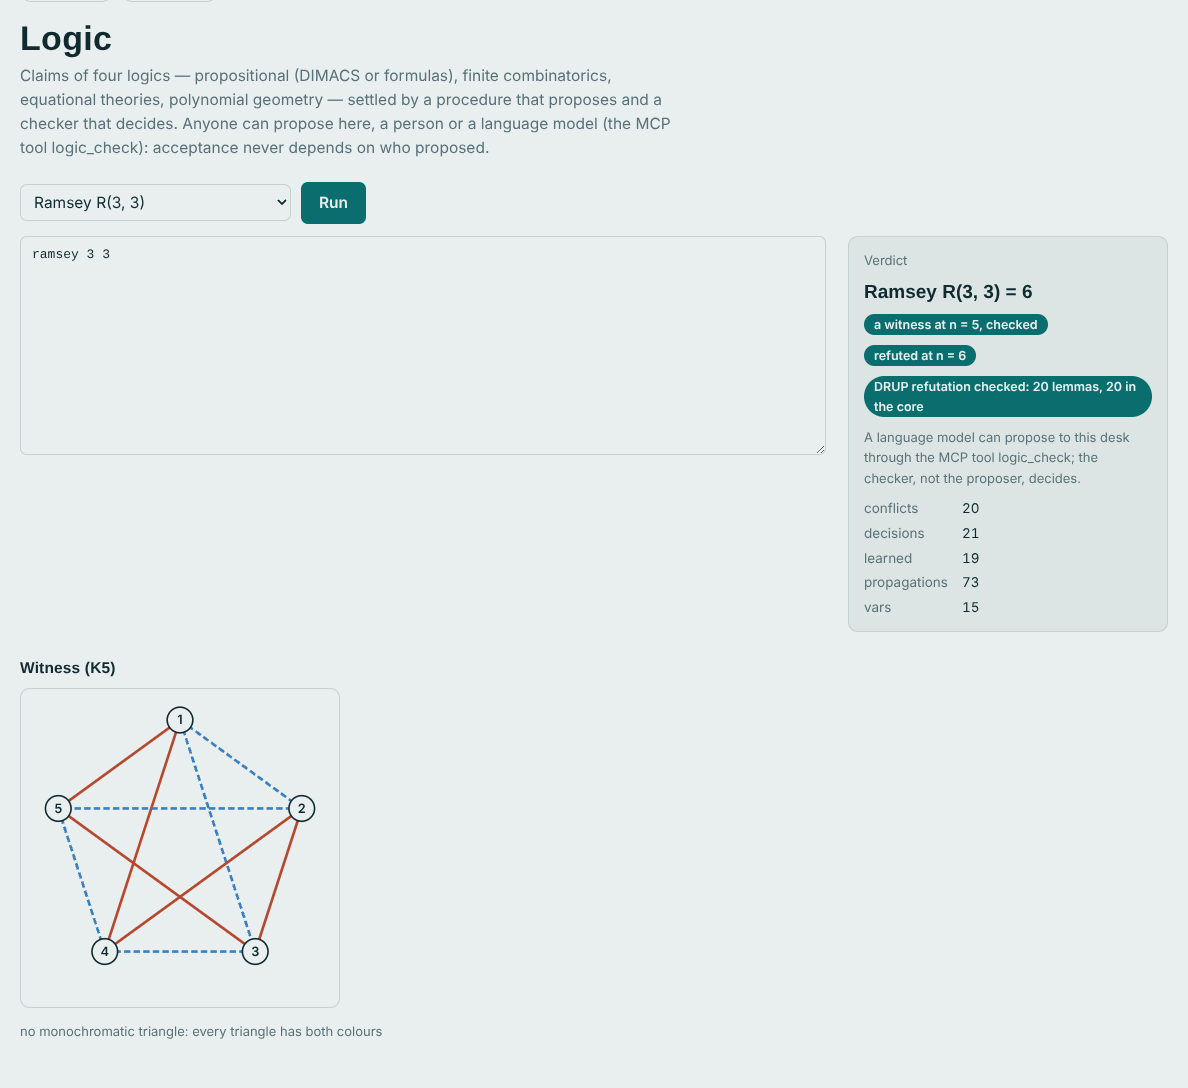
\includegraphics[width=0.78\textwidth]{figuras/console-logica.png}
\caption{A mesa de lógica no console: a afirmação, a decisão e a prova conferível.}
\label{fig:logica}
\end{figure}

\paragraph{Limite.} O padrão exige que exista um verificador mais simples que a busca. Isso vale para problemas em NP e para a otimização convexa (dualidade), mas não para toda pergunta: ``esta estratégia vai dar lucro?'' não tem certificado --- tem, no máximo, portões que dizem quando um \textit{backtest} é indistinguível de ruído (\autoref{sec:fin-backtest}).

% ----------------------------------------------------------------------------
\section{Repetir é verificar}\label{sec:inov-repetir}

\begin{ficha}{Ficha 8 --- Execuções que são objetos de prova}
\textbf{O quê.} Agentes, grafos do estúdio, sessões de bolsa e arquivos salvos cuja execução produz um diário encadeado por \textit{hash}, fechado por uma raiz de Merkle e atestado, de modo que reexecutar é a forma de conferir.\\
\textbf{Para quem.} Quem precisa auditar o que um agente ou um processo automatizado fez.\\
\textbf{Para que.} Para que ``o que aconteceu'' seja recalculável, não narrado.\\
\textbf{Por que.} Porque, com bits canônicos, toda decisão local é re-derivável em qualquer substrato.\\
\textbf{Como.} Diário gravado antes de cada passo; repetição que recalcula sem agir; retomada do disco sem repetir ações; apagamento por titular.
\end{ficha}

A rodada 0.13 estende a ideia ao mercado: a mesma semente de uma sessão de bolsa reproduz \emph{a mesma cabeça de hash} do diário, e outra semente, outra cabeça. Os arquivos salvos das mesas passam a ser \emph{assinados} (Ed25519 sobre \code{"vapor-archive-v1\textbackslash n"} seguido do manifesto), e um manifesto reescrito é recusado.

% ----------------------------------------------------------------------------
\section{Primeiros princípios: as inversões}\label{sec:inov-inversoes}

As inovações acima têm uma raiz comum: cada uma inverte uma suposição que a prática trata como dada. A \autoref{tab:inversoes} as reúne.

\begin{table}[htbp]
\centering
\caption{As suposições usuais e a inversão do \vapor{}}\label{tab:inversoes}
\small
\begin{tabularx}{\textwidth}{@{}XX@{}}
\toprule
\textbf{suposição usual} & \textbf{inversão}\\
\midrule
reprodutibilidade custa desempenho & o paralelismo vem de saídas independentes; a ordem da soma é fixa e de graça\\
o compilador é confiável ou é provado inteiro & o compilador é não confiável; uma fase difícil é conferida por um verificador provado\\
código gerado roda no processo do \textit{runtime} & nenhum byte gerado roda na VM\\
o certificado diz onde rodar & o certificado diz o trabalho; cada nó decide\\
um modelo é aceito porque carrega & um modelo é aceito porque cumpre um contrato conferido contra a referência\\
uma saída boa é uma saída plausível & uma saída boa passou num juiz que tem poder (controle)\\
um \textit{backtest} é um modelo da bolsa & o \textit{backtest} é o código da bolsa (\autoref{sec:fin-sessao})\\
antecipação se evita com disciplina & antecipação se \emph{certifica} ausente, por invariância de prefixo (\autoref{sec:fin-backtest})\\
arbitragem se estima & arbitragem se decide, em racionais, pelo lema de Farkas (\autoref{sec:fin-arbitragem})\\
\bottomrule
\end{tabularx}
\end{table}

\begin{doutorado}
\textbf{Uma teoria dos controles.} A prática de acompanhar cada verificação de um controle que ``deveria ser recusado'' lembra o \textit{mutation testing} e a análise de poder estatístico, mas não é nenhum dos dois: o controle é \emph{escolhido} para representar o erro mais plausível (esquecer o termo de Itô, contar dias corridos em vez de úteis, normalizar pela amostra inteira). Falta uma teoria que diga quais controles bastam para dar a um conjunto de verificações uma garantia de cobertura --- por exemplo, uma noção de ``controle adversarial mínimo'' por classe de erro, com cotas sobre a probabilidade de um defeito passar despercebido. O \vapor{} oferece um corpus de 170 pares (verificação, controle) em domínios variados como ponto de partida empírico.
\end{doutorado}
